%!TEX program = xelatex

\documentclass[cn,black,9pt,normal]{elegantnote}
\usepackage{float}
\usepackage{hyperref}


%\newcommand{\upcite}[1]{\textsuperscript{\textsuperscript{\cite{#1}}}}

\title{数码摄影作业(02)不同亮度的两张照片\\\small{同济大学医学楼}}
\author{姓名:姜文渊\\学号:1951510}
%\institute{School of Life Science, Tongji University}
%\version{1.00}
\date{2021年3月24日}

\begin{document}

\maketitle


\section*{拍摄条件及使用器材简介}

下面两张照片是学生所摄的同济大学医学楼,拍摄时间大致为晚上十点,使用的相机为佳能M200,镜头为\texttt{EF-M15-45mm f/3.5-6.3 IS STM}。

\section{所摄照片}
\begin{figure}[H]
    \centering
    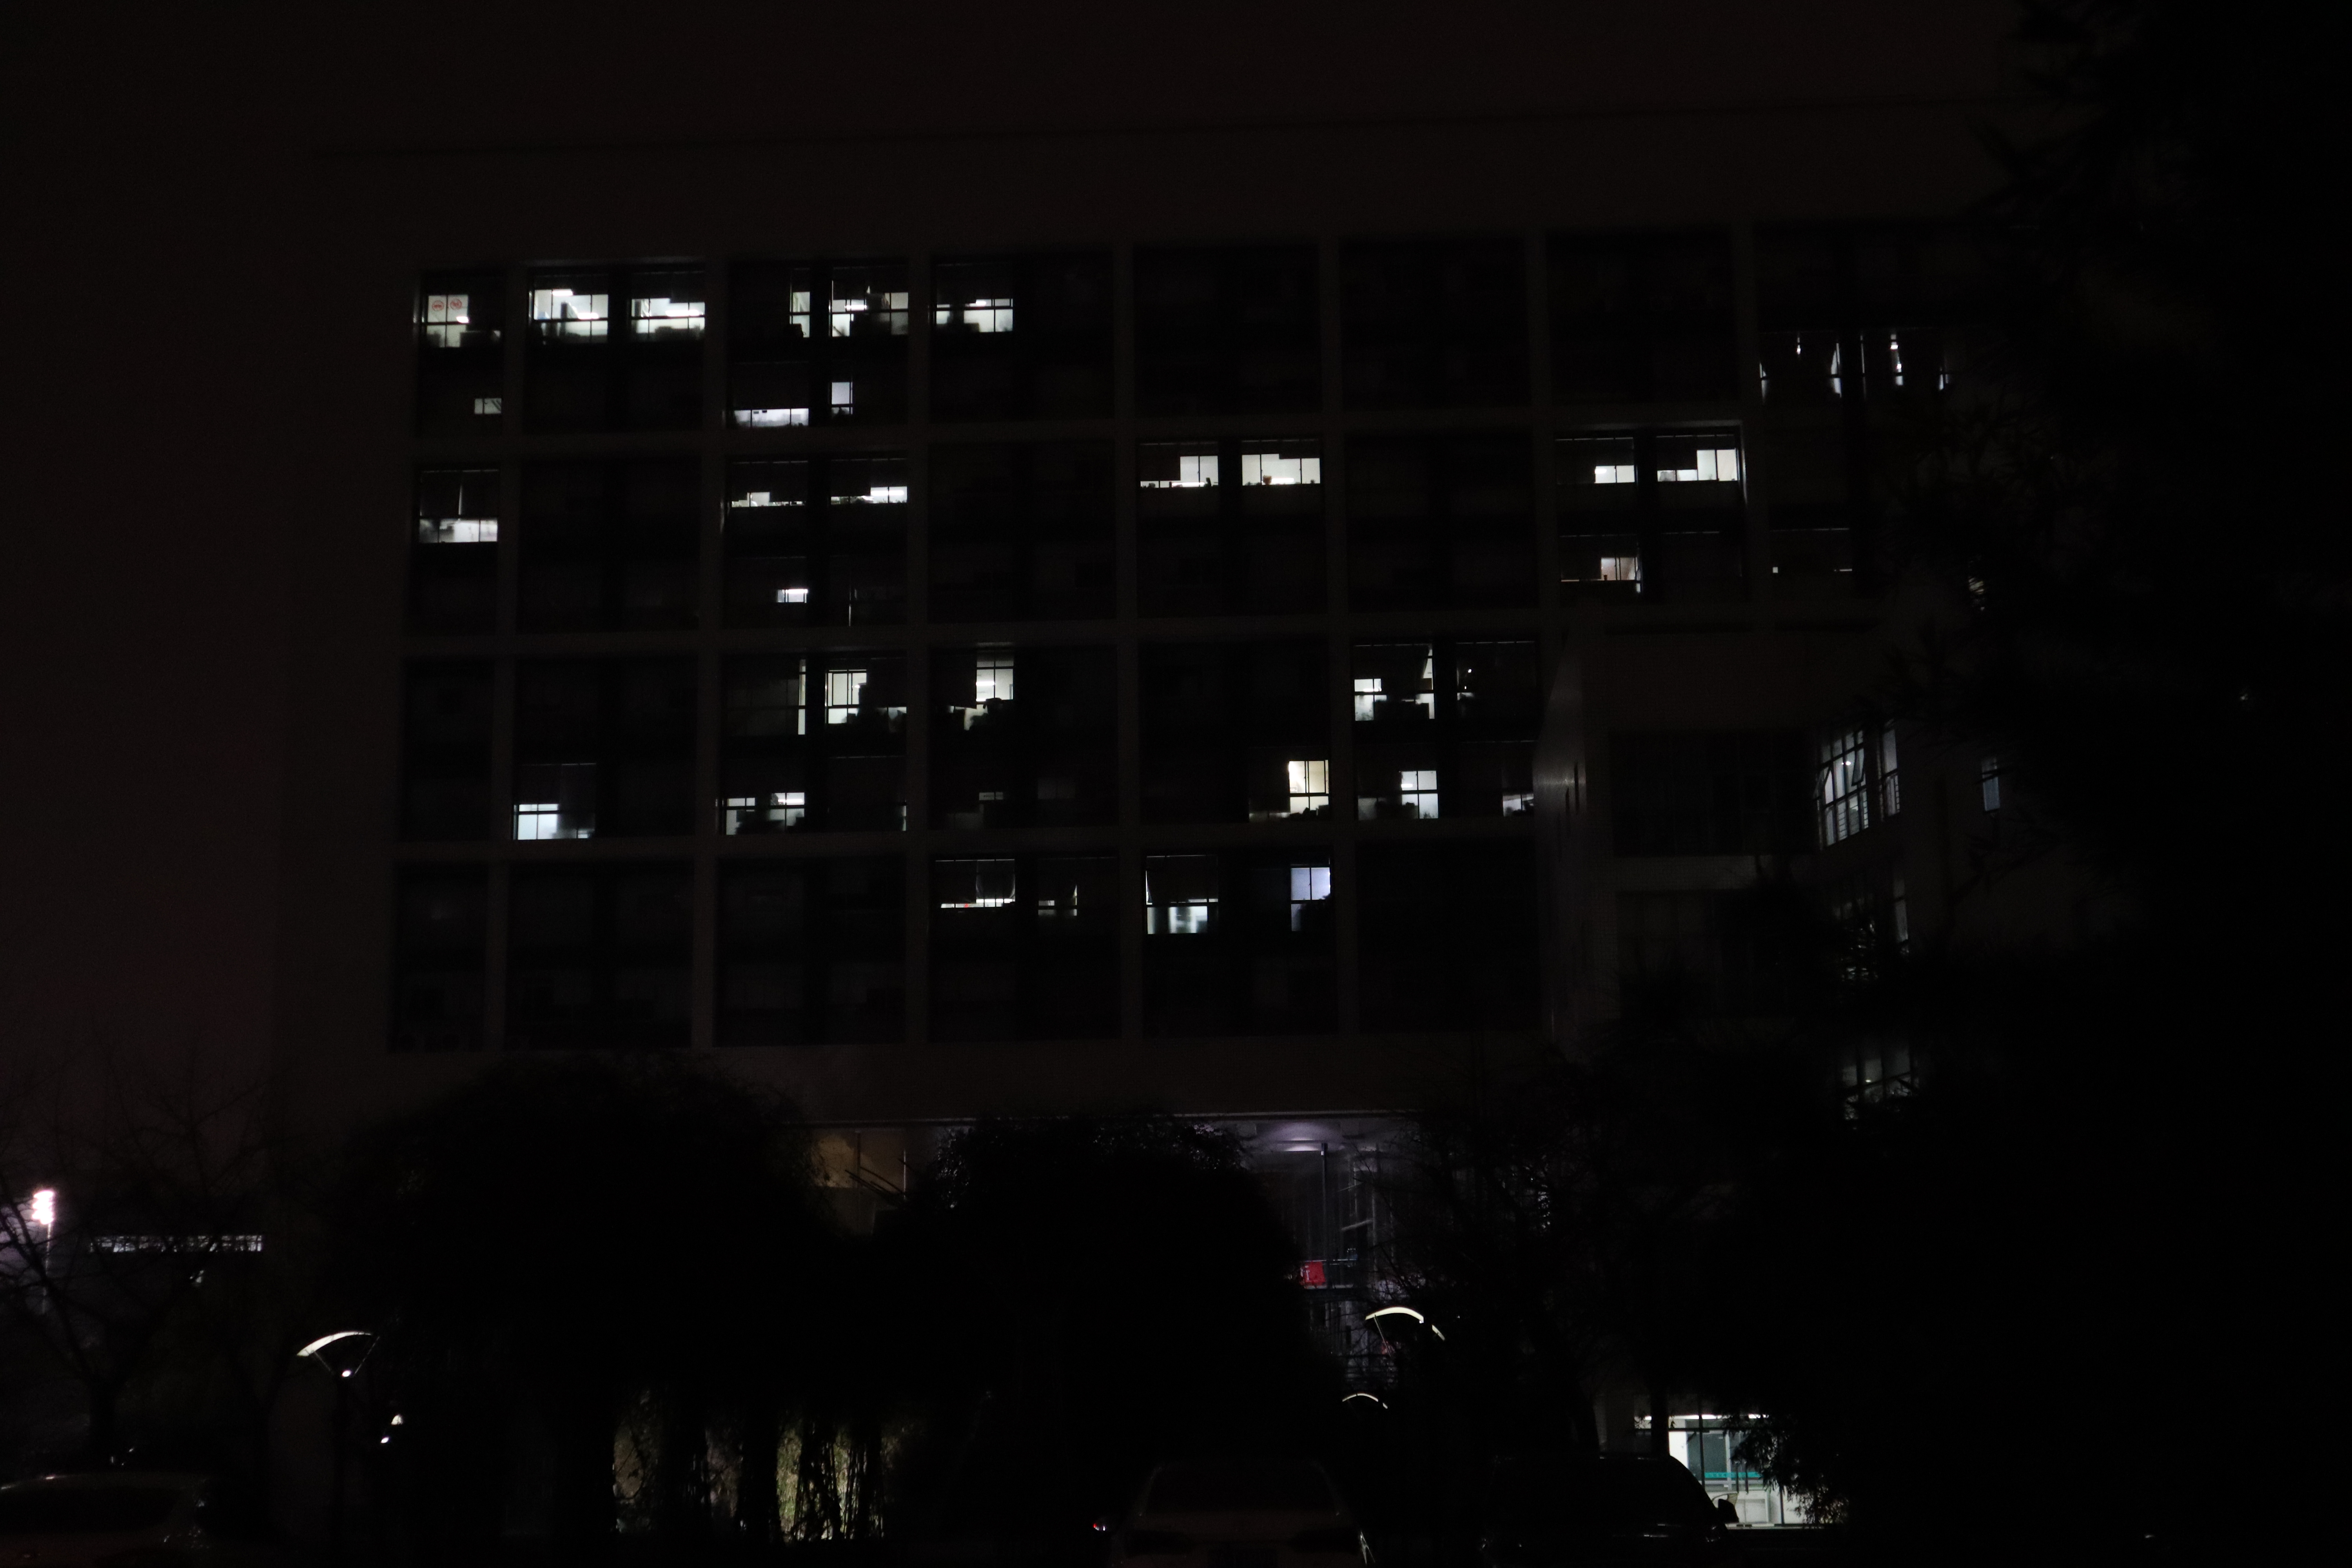
\includegraphics[width=1\textwidth]{IMG_0405.JPG}
    \caption{28mm 1/30 F5.0 ISO 3200}
    \label{F-01}
\end{figure}

上面的照片ISO与快门时间均较小,画面偏暗,突出表现夜晚医学楼众多实验室仍在认真工作的情景,但医学楼的建筑细节就不容易展现。
\section{所摄照片}
\begin{figure}[H]
    \centering
    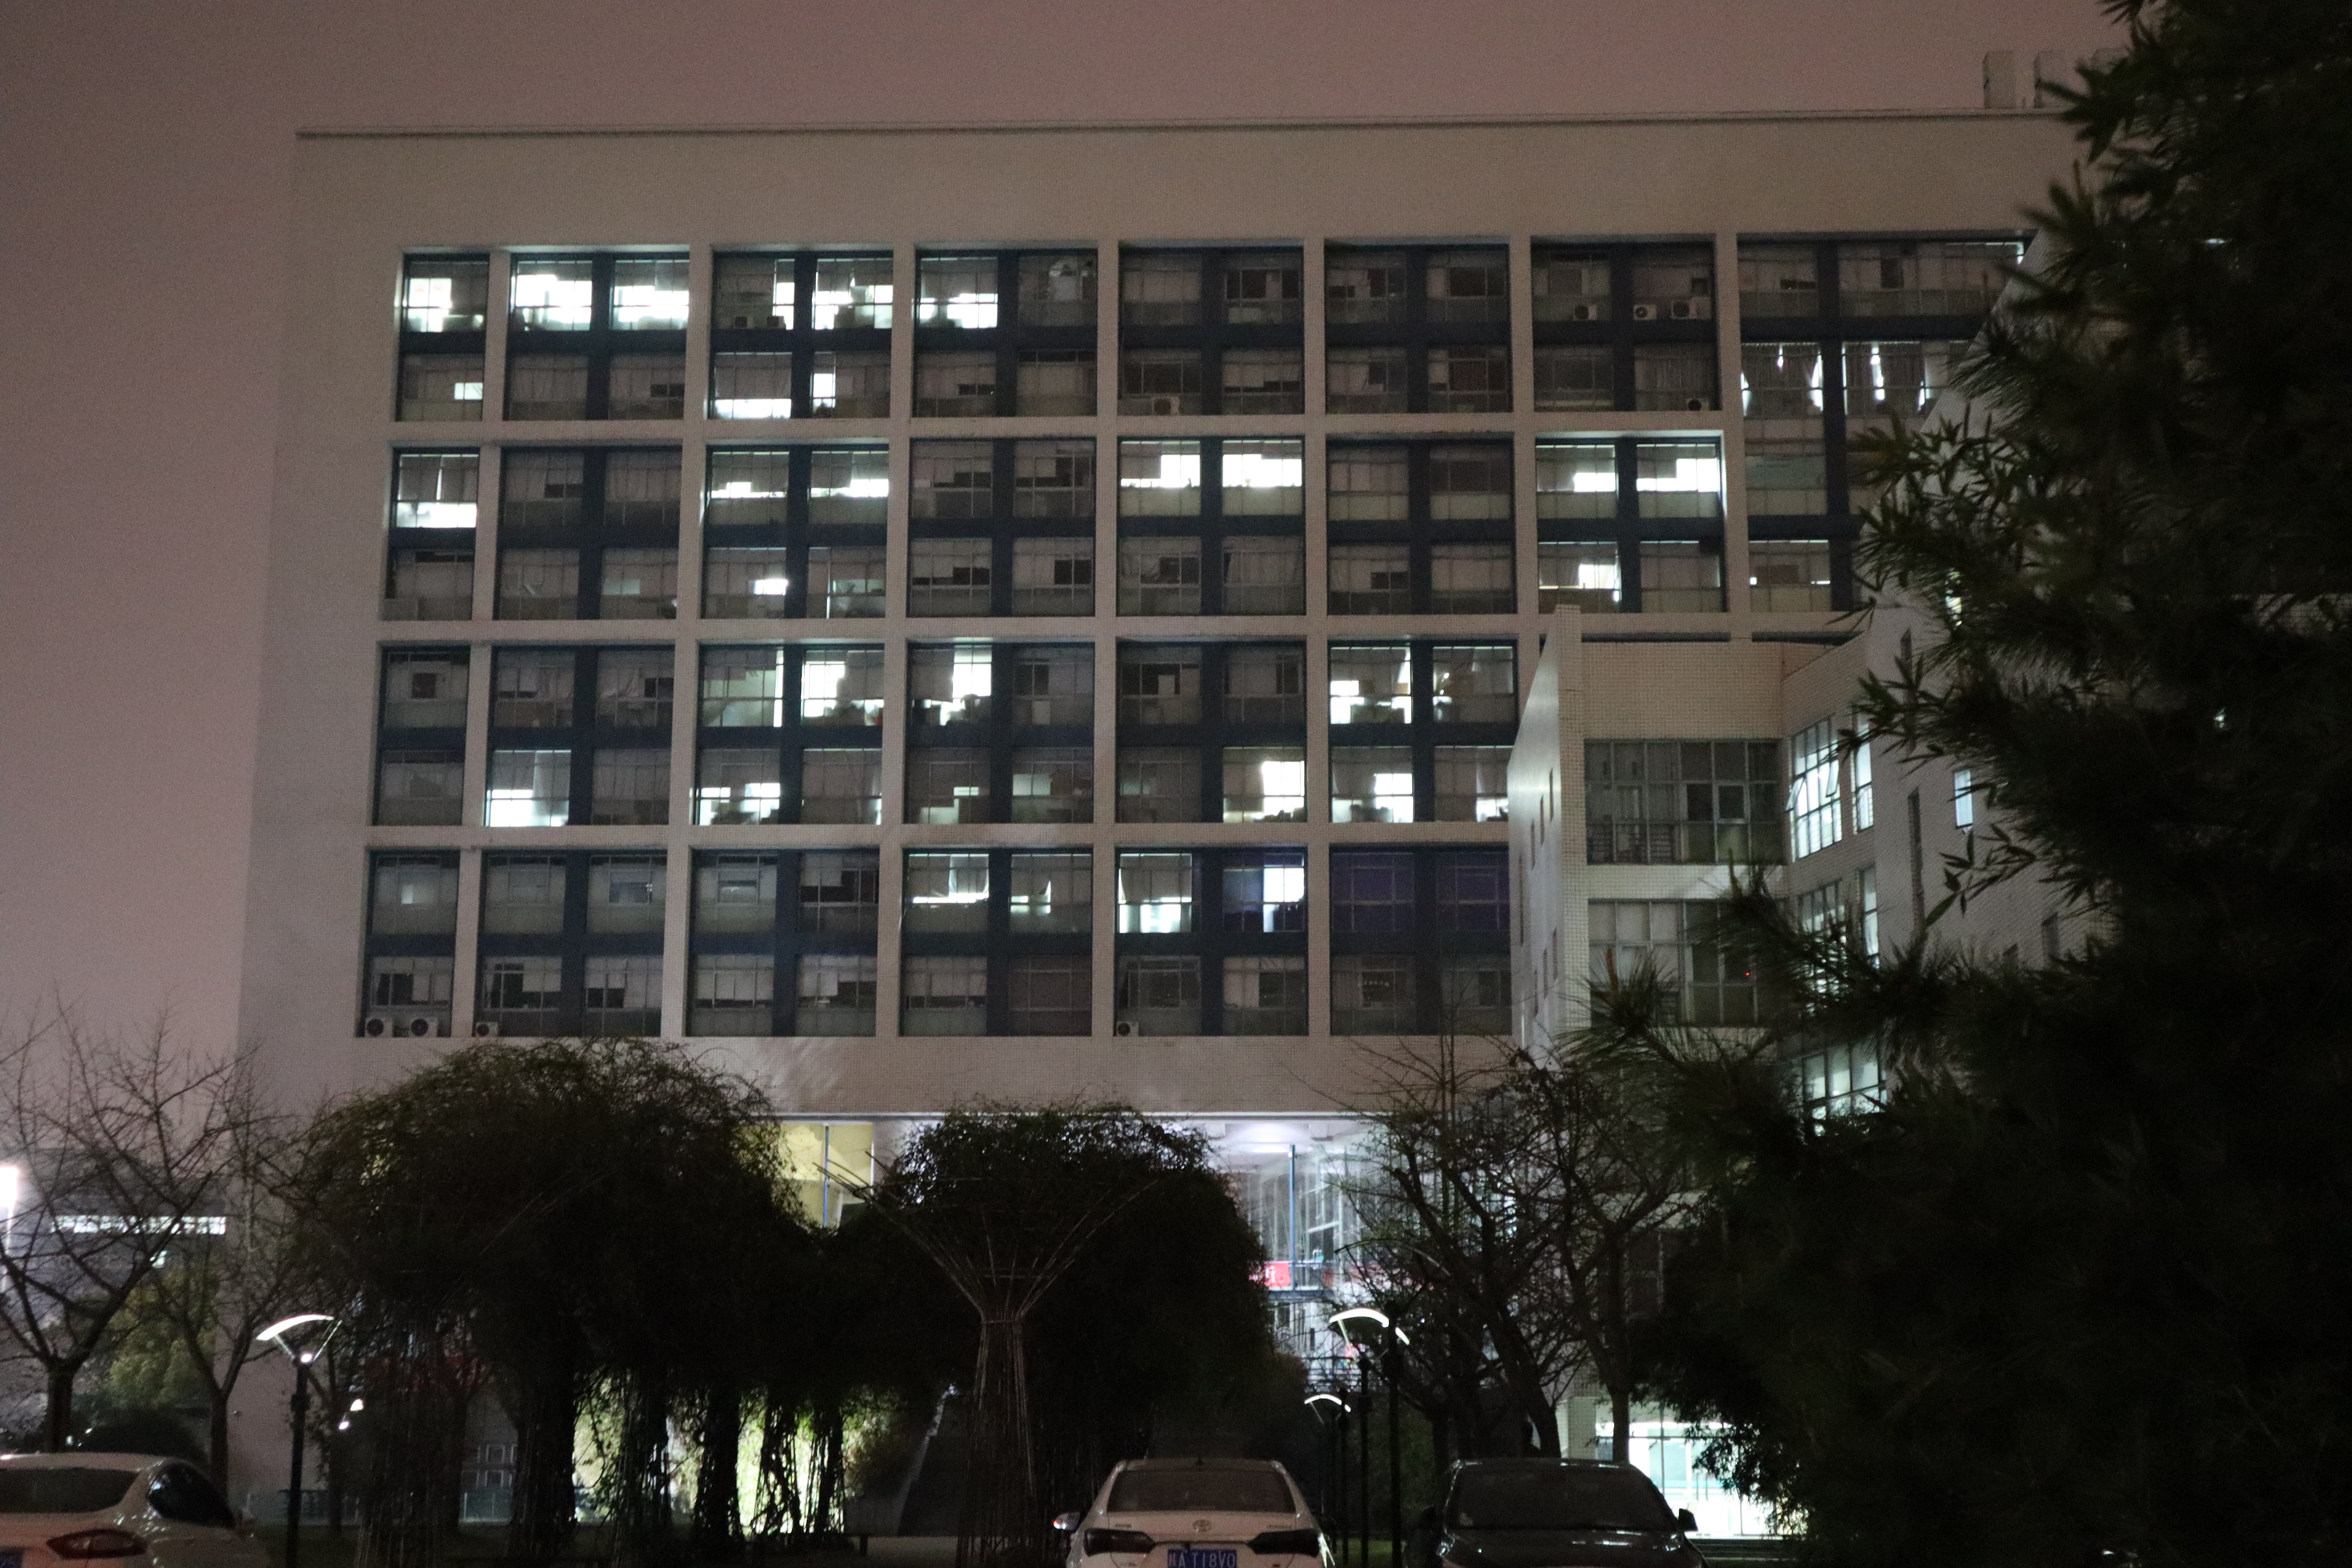
\includegraphics[width=1\textwidth]{IMG_0406.JPG}
    \caption{28mm 1/6 F5.0 ISO 6400}
    \label{F-02}
\end{figure}

而这张照片较为明亮,可以展现出医学楼建筑的外观和细节,但无法体现深夜众多教授和研究生进行实验工作但辛勤情景。

%\bibstyle{unsrt}
%\bibliography{references}{}
\end{document}
